\documentclass[10pt]{book}

\usepackage[letterpaper,top=2.5cm,bottom=2.5cm,left=2.5cm,right=2.5cm]{geometry}
\usepackage[utf8]{inputenc}
\usepackage{graphicx}
\usepackage{multicol}
\usepackage[normalem]{ulem}
\usepackage{float}
\usepackage[usenames,dvipsnames]{color}
\usepackage{amsmath}
\usepackage[table]{xcolor}
\usepackage{xspace}
\usepackage{fancyhdr}
\usepackage[nolist]{acronym}
\usepackage{listings}
% note sure after here
\usepackage{makeidx}
\usepackage[UKenglish]{isodate}
\usepackage{ifthen}
\usepackage{textcomp}
\usepackage{alltt}
\usepackage{ifpdf}
\ifpdf
\usepackage[pdftex,
            pagebackref=true,
            colorlinks=true,
            linkcolor=blue,
            unicode
           ]{hyperref}
\else
\usepackage[ps2pdf,
            pagebackref=true,
            colorlinks=true,
            linkcolor=blue,
            unicode
           ]{hyperref}
\usepackage{pspicture}
\fi
\usepackage{sectsty}
\usepackage{mathptmx}
\usepackage[scaled=.90]{helvet}
\usepackage{courier}
\usepackage[titles]{tocloft}
\usepackage{prettyref}
\usepackage{mdwlist}
\usepackage{enumitem}
\usepackage{framed}
\usepackage{pbox} 
\usepackage{draftcopy}
\usepackage{draftwatermark}
\usepackage{wrapfig}
\usepackage{caption}
\usepackage{subcaption}


\definecolor{ListingBG}{rgb}{0.91,0.91,0.91}
\definecolor{shadecolor}{rgb}{0.92,0.92,0.92}


\renewcommand{\chaptername}{Chapter} 
\renewcommand{\appendixname}{Annex} 

% Place some penalty for doing the break
% The penalty for a ``\gb'' should be greater than a \hyphenpenalty.
% \hyphenpenalty is 50 in plain.tex.
\def\gb{\penalty10000\hskip 0pt plus 8em\penalty4800\hskip 0pt plus-8em%
\penalty10000}

% This macro enables that all "_" (underscore) characters in the pfd
% file are searchable, and that cut&paste will copy the "_" as underscore. 
% Without the following macro, the \_ is treated in searches and cut&paste
% as a " " (space character). 
% This macro does not modify the behavior of _ in math or in verbatim 
% environments. In verbatim environments, the "_" is always treated
% as a searchable character.
%
\DeclareRobustCommand{\_}{\texttt{\char`\_}} 
% 

\def\colorswapnt{\colorlet{saved}{.}\color{ForestGreen}}
\def\colorswapot{\colorlet{saved}{.}\color{red}}
\def\prevcolor{\color{saved}}

\newcommand{\newtext}[1]{\textcolor{ForestGreen}{#1}}
\newcommand{\oldtext}[1]{\textcolor{red}{\sout{#1}}}
\newcommand{\insertDocVersion}{1.0}
\newcommand{\qcor}{\emph{QCOR}\xspace}
\newcommand{\FUNC}[1]{\textit{#1}}
\newcommand{\VAR}[1]{\textit{#1}}
\newcommand{\CONST}[1]{\textit{#1}}
\newcommand{\const}[1]{\protect\gb\protect{\textsf{\small #1}}\index{CONST:#1}}
\newcommand{\CorCpp}{\textit{C/C++}\xspace}
\newcommand{\Python}{\textit{Python}\xspace}
\newcommand{\Clang}{\textit{C}\xspace}
\newcommand{\Cpp}{\textit{C++}\xspace}
\newcommand{\Celev}{\textit{C11}\xspace}
\newcommand{\TYPE}{\emph{TYPE}}
\newcommand{\TYPENAME}{\emph{TYPE}}
\newcommand{\ColHead}[1]{\textbf{#1}}
\newcommand{\DATATYPENAME}[1]{\emph{#1}}
\newcommand{\METHODNAME}[1]{\emph{#1}}
\newcommand{\VARTYPE}[1]{\textit{#1}}
\newcommand{\SIZE}{\emph{SIZE}}

\newcommand{\source}{\textit{source}}
\newcommand{\target}{\textit{target}}
\newcommand{\dest}{\textit{dest}}

\begin{acronym}
\acro{API}{\lowercase{a}pplication \lowercase{p}rogramming \lowercase{i}nterface}
\acro{ORNL}{Oak Ridge National Laboratory}
\acro{DOE}{Department of Energy}
\acro{NISQ}{Noisy Intermediate Scale Quantum}
\acro{HQCC}{Hybrid Quantum Classical Computation}
\end{acronym}


%
% This is used to put line numbers on plain pages.  Used in draft.tex
%
\makeatletter

\def\withlinenumbers{\relax
  \def\@evenfoot{\hbox to 0pt{\hss\LineNumberRuler\hskip 1.5pc}\hfil}\relax
  \def\@oddfoot{\hfil\hbox to 0pt{\hskip 1.5pc\LineNumberRuler\hss}}}

\def\LineNumberRuler{\vbox to 0pt{\vss\normalsize \baselineskip13.6pt
    \lineskip 1pt \normallineskip 1pt \def\baselinestretch{1}\relax
    \LNR{1}\LNR{2}\LNR{3}\LNR{4}\LNR{5}\LNR{6}\LNR{7}\LNR{8}\LNR{9}
    \LNR{10}\LNR{11}\LNR{12}\LNR{13}\LNR{14}
        \LNR{15}\LNR{16}\LNR{17}\LNR{18}\LNR{19}
    \LNR{20}\LNR{21}\LNR{22}\LNR{23}\LNR{24}
        \LNR{25}\LNR{26}\LNR{27}\LNR{28}\LNR{29}
    \LNR{30}\LNR{31}\LNR{32}\LNR{33}\LNR{34}\LNR{35}
        \LNR{36}\LNR{37}\LNR{38}\LNR{39}
    \LNR{40}\LNR{41}\LNR{42}\LNR{43}\LNR{44}
        \LNR{45}\LNR{46}\LNR{47}\LNR{48}
    \vskip 31pt}}
\def\LNR#1{\hbox to 1pc{\hfil\tiny#1\hfil}}

\def\ps@plainwithlinenumbers{\let\@mkboth\@gobbletwo
     \def\@oddhead{}
     \def\@oddfoot{\hfil\rm\thepage\hfil
       \hbox to 0pt{\hskip 1.5pc\LineNumberRuler\hss}}
     \def\@evenhead{}
     \def\@evenfoot{\hbox to 0pt{\hss
     \LineNumberRuler\hskip 1.5pc}\rm\hfil\thepage\hfil}}

    % Contents is done with \chapter*{Contents}, so we need to turn off the
    % line numbers in this case.  Easiest to look at def

\newwrite\chappages
\immediate\openout\chappages=chappage.txt
\def\writespace{ }

\def\incontents{0}
\newif\ifcontents
\contentsfalse
\def\chapter{\clearpage \ifcontents\else\thispagestyle{plainwithlinenumbers}\fi
        \write\chappages{Chapter \thechapter\writespace - \the\count0}
        \global\@topnum\z@ \@afterindentfalse \secdef\@chapter\@schapter}

\makeatother

%
% End this is used to put line numbers on plain pages.  Used in draft.tex
%

%
% Use Sans Serif font for sections, etc.
%
\makeatletter
\def\section{\@startsection {section}{1}{\z@}{-3.5ex plus -1ex minus 
-.2ex}{2.3ex plus .2ex}{\Large\sf}}
\def\subsection{\@startsection{subsection}{2}{\z@}{-3.25ex plus -1ex minus 
-.2ex}{1.5ex plus .2ex}{\large\sf}}
\def\subsubsection{\@startsection{subsubsection}{3}{\z@}{-3.25ex plus 
-1ex minus -.2ex}{1.5ex plus .2ex}{\normalsize\sf\bf}}
\def\paragraph{\@startsection {paragraph}{4}{\z@}{3.25ex plus 1ex 
minus .2ex}{-1em}{\normalsize\sf}}
\makeatother
%
% End use Sans Serif font for sections, etc.  S. Otto
%


%
% This section is for example code listings
%
\definecolor{gray}{rgb}{0.92,0.92,0.92}

\lstset{ % set defaults for languages not otherwise defined
  breakatwhitespace=false,         % sets if automatic breaks should only happen at whitespace
  basicstyle=\ttfamily\footnotesize,
  breaklines=true,                 % sets automatic line breaking
  escapeinside={|}{|},          % if you want to add LaTeX within your code
  extendedchars=true,              % lets you use non-ASCII characters; for 8-bits 
                                   % encodings only, does not work with UTF-8
  keepspaces=true,                 % keeps spaces in text, useful for keeping indentation of code 
                                   % (possibly needs columns=flexible)
  morekeywords={*,...},            % if you want to add more keywords to the set
  showspaces=false,                % show spaces everywhere adding particular underscores; 
                                   % it overrides 'showstringspaces'
  showstringspaces=false,          % underline spaces within strings only
  showtabs=false,                  % show tabs within strings adding particular underscores
}

\def\StandardListing {
  \lstset {
    breakatwhitespace=false,         % sets if automatic breaks should only happen at whitespace
    basicstyle=\ttfamily\footnotesize,
    breaklines=true,                 % sets automatic line breaking
    escapeinside={\%*}{*)},          % if you want to add LaTeX within your code
    extendedchars=true,              % lets you use non-ASCII characters; for 8-bits 
                                     % encodings only, does not work with UTF-8
    keepspaces=true,                 % keeps spaces in text, useful for keeping
                                     % indentation of code (possibly needs columns=flexible)
    morekeywords={*,...},            % if you want to add more keywords to the set
    showspaces=false,                % show spaces everywhere adding particular underscores; 
                                     % it overrides 'showstringspaces'
    showstringspaces=false,          % underline spaces within strings only
    showtabs=false,                  % show tabs within strings adding particular underscores
    backgroundcolor=\color{gray}, 
  }
}

\def\ProgramNumberedListing {
  \StandardListing
  \lstset {
    numbers=left,
    numberstyle=\footnotesize
  }
}

\newcommand{\numberedlisting}[2] {
  \ProgramNumberedListing
  \lstinputlisting[#1]{#2}
  \StandardListing
}

\newcommand{\outputlisting}[2] {
\begin{minipage}{\linewidth}
\vspace{0.1in}
  \lstinputlisting[#1]{#2}
  \StandardListing
\vspace{0.1in}
\end{minipage}
}


%
% End this section is for example code listings
%

%
% Library API description template commands
%

\newcommand{\apisummary}[1]{
    #1
\hfill
}

\newenvironment{apidefinition}{
\begin{description}
\item[SYNOPSIS] \hfill \\ \\ 
\vspace{-2em}
}
{
\end{description}
}

\lstnewenvironment{C11synopsis}
{ 
  \textbf{C11:} 
  \lstset{language={C++}, backgroundcolor=\color{gray}, lineskip=2pt,
  morekeywords={size_t, TYPE}, aboveskip=0pt, belowskip=0pt}}{}


\lstnewenvironment{Cppsynopsis}
{ 
  \textbf{C++:} 
  \lstset{language={C++}, backgroundcolor=\color{gray}, lineskip=2pt,
  morekeywords={size_t, TYPE}, aboveskip=0pt, belowskip=0pt}}{}


\lstnewenvironment{Csynopsis}
{ 
  \textbf{C:} 
  \lstset{language={C}, backgroundcolor=\color{gray}, lineskip=2pt,
  morekeywords={size_t, TYPE, TYPENAME, SIZE}, aboveskip=0pt, belowskip=0pt}}{}


\lstnewenvironment{CppCsynopsis}
{ 
  \textbf{C/C++:} 
  \lstset{language={C}, backgroundcolor=\color{gray}, lineskip=2pt,
  morekeywords={size_t, TYPE, TYPENAME, SIZE}, aboveskip=0pt, belowskip=0pt}}{}

\lstnewenvironment{CsynopsisST}
{ 
  \textbf{C/C++:} 
  \color{red}  
  {\lstset{language={C}, backgroundcolor=\color{gray}, lineskip=2pt,
  morekeywords={size_t}, aboveskip=0pt, belowskip=0pt}}
  }
  {}
  
\lstnewenvironment{Fsynopsis}
{ \textbf{FORTRAN:} 
  \lstset{language={Fortran}, backgroundcolor=\color{gray}, lineskip=3pt,
  deletekeywords=[2]{STATUS},
  deletekeywords=[3]{LOG}, aboveskip=0pt,
  belowskip=0pt}}{}

\newenvironment{apiarguments}{
\newcommand{\apiargument}[3]{
\begin{tabular}{p{2cm} p{2cm} p{10cm}}
\textbf{##1} & \textit{##2} & {##3} \\ 
\end{tabular}
}
\hfill
\item[DESCRIPTION] \hfill 

\begin{description}
\item[Arguments] \hfill \\
}
{
\hfill
\end{description}
}

\newcommand{\apidescription}[1]{
\begin{description}
\vspace{-1em}
\item[API description] \hfill \\ 
    #1
\hfill
}

\newcommand{\typedescription}[1]{
\begin{description}
\vspace{-1em}
\item[Datatype description] \hfill \\ 
    #1
\hfill
}

\newcommand{\structdescription}[1]{
\begin{description}
\vspace{-1em}
\item[Data structure description] \hfill \\ 
    #1
\hfill
}

\newcommand{\apidesctable}[4] {\hfill \\ #1 \\ \\
    \begin{tabular}{p{5cm} p{9cm}}
       \hline
       #2 & #3 \\
       \hline \tabularnewline
       \end{tabular}\\
        #4
}  

\newcommand{\apireturnvalues}[1]{
\hfill 
\item[Return Values] \hfill \\
    #1
\\
\hfill
}

\newcommand{\apitablerow}[2]{
 \begin{tabular}{p{5cm} p{9cm}}
 #1 & #2 \tabularnewline
  \end{tabular}\\
}

\newcommand{\apinotes}[1]{
\item[Notes] \hfill \\
    #1
\hfill \\
\end{description}
}

\newcommand{\apiimpnotes}[1]{
\begin{description}
\item[Note to implementors] \hfill \\
    #1
\hfill \\
\end{description}
}

\newenvironment{apiexamples}{
\newcommand{\apicexample}[3]{
    ##1
    \lstinputlisting[language={C}, tabsize=2,
    basicstyle=\ttfamily\footnotesize, morekeywords={size_t}]{##2}
    ##3 }
\newcommand{\apicppexample}[3]{
    ##1
    \lstinputlisting[language={C++}, tabsize=2,
    basicstyle=\ttfamily\footnotesize, morekeywords={size_t}]{##2}
    ##3 }
\newcommand{\apifexample}[3]{
    ##1
    \lstinputlisting[language={Fortran}, tabsize=2,
    basicstyle=\ttfamily\footnotesize, deletekeywords={TARGET}]{##2}
    ##3 }
\vspace{-2pt}
\item[EXAMPLES] \hfill \\
\vspace{-2pt}
}
{
}

%
% End library API description template commands
%


\makeindex

\begin{document}

\hypersetup{pageanchor=true,citecolor=blue}

% Set header/footer for opening content
\pagestyle{fancy}
\fancyhead{}
\fancyhead[LE,LO]{\insertDocVersion}
\fancyhead[CO,CE]{--- DRAFT ---}
\SetWatermarkText{DRAFT}
\SetWatermarkScale{1}
\fancyfoot[CE,CO]{\thepage} %affects page numbering for the first pages, 
                            %except the first ToC page

\pagenumbering{roman} %sets coverpage and toc page numbers to roman numerals

\thispagestyle{empty}
\begin{center}
\textbf{\Huge \qcor}
\par
\end{center}
\begin{center}
\textbf{\LARGE Application Programming Interface}\\
%\includegraphics[scale=0.65]{figures/}\\
%\url{}
\par
\end{center}

\begin{center}
Version \insertDocVersion
\par
\end{center}

\vspace{0.5in}
\begin{center}
\today
\end{center}

\vspace{0.5in}

\vfill{}

\section*{Developed by}
The Software Stack and Algorithms for Automating Quantum-Classical Computing Project \\
\url{https://qcor.ornl.gov}
%\begin{itemize}
%\item Put team/project name here\\
%  \url{} 
%\end{itemize}
\pagebreak{}

\section*{Sponsored by}
\begin{itemize}
\item \ac{DOE}\\
  \url{https://www.energy.gov}
\item \ac{ORNL}\\
  \url{http://www.ornl.gov/} 
\end{itemize}

\section*{Authors and Collaborators}
\begin{itemize}
\item Eugene Dumitrescu, \ac{ORNL}
\item Chung-Hsing Hsu, \ac{ORNL}
\item Tyler Kharazi, \ac{ORNL}
\item Pavel Lougovski, \ac{ORNL}
\item Alexander McCaskey, \ac{ORNL}
\item Tiffany M. Mintz, \ac{ORNL}
\item Shirley V. Moore, \ac{ORNL}
\item Sarah Powers, \ac{ORNL}
\item Zak Webb, \ac{ORNL}
\end{itemize}

\date{\today}

\section*{Acknowledgements}





\setcounter{tocdepth}{4}
\setcounter{secnumdepth}{3}
\tableofcontents

\mainmatter  % included for use of documenttype 'book' 


% Set header/footer for main content
\pagestyle{fancy}   %replacing {headings} with {fancy} for customization 
\withlinenumbers    %adds line numbers to edges of normal pages
\fancyhf{}
\fancyhead[RE, LO]{\rightmark}
\fancyhead[RO, LE]{\thepage}
\renewcommand{\headrulewidth}{0pt}
\renewcommand{\thesection}{\arabic{section}}

{ %using setlength to force standardized spacing, if needed
% this command is ended in backmatter.tex
%\setlength{\baselineskip}{3pt plus 3pt minus 3pt}

\setlength{\parskip}{3pt}






%\section{The \qcor Effort}\label{subsec:qcor_effort}
%


\section{Programming Model Overview}\label{subsec:programming_model}
In the \ac{HQCC} paradigm, a classically hard computational task is broken up into a sequence of quantum and classical subtasks. The former are designed such that a quantum device can efficiently evaluate them. The latter are chosen so as to be solvable by a classical computer. 
\qcor leverages the \ac{HQCC} paradigm to develop a programming model that enables a sequence of quantum and classical subtasks to be implemented cooperatively in a single application. The \qcor programming model is a single-source heterogeneous programming model that allows quantum kernels to be implemented within a \Clang or \Cpp application. \qcor's language extensions allow quantum kernels to be constructed using high level \CorCpp syntax via library calls and directives. The library calls and directives are designed to satisfy the requirements for \ac{HQCC} algorithms, but could in principle be used for more general schemes, e.g. those involving feed-forward logic. 


\section{Memory Model}\label{subsec:memory_model}
The \qcor memory model assumes that the host memory and quantum control system memory are discrete memory spaces with explicit and implicit memory accesses between the two memory spaces.  
All memory access is explicit on the host device -- i.e., there is a library call or directive expressed in the code by the programmer. On the other hand, memory allocation on and data transfer to the quantum device are implicitly managed by the compiler. For example, an explicit allocation of memory for ``quantum results'' also implicitly requires the same memory for "quantum results" to be accessible on the quantum device. In addition, the host must explicitly allocate memory to create instances of objective functions and observables, and these are implicitly allocated as quantum registers to evaluate the observable on the quantum side. 

The discrete memory spaces in the \qcor memory model support shared and distributed memory between the host and quantum system. 
When the memory spaces are distributed, a copy of the allocated memory exists in both the host and quantum system address spaces.  
Memory that is written by the quantum system is updated in the host memory address space with library calls on the host. 
Memory written by the host is also updated on the quantum system with library calls on the host.  
When the memory space is shared between the host device and quantum system, we assume that there is an allocatable block of memory where the physical location of the memory is abstracted away, and that a block of memory allocated in this shared space is accessible by both the host and the quantum device. Because this block of memory is accessible by both systems, the library calls that access and update memory do not require a memory copy. Figure \ref{fig:mem_model} provides an illustration of the memory system.

\begin{figure*}[ht]
 \centering
  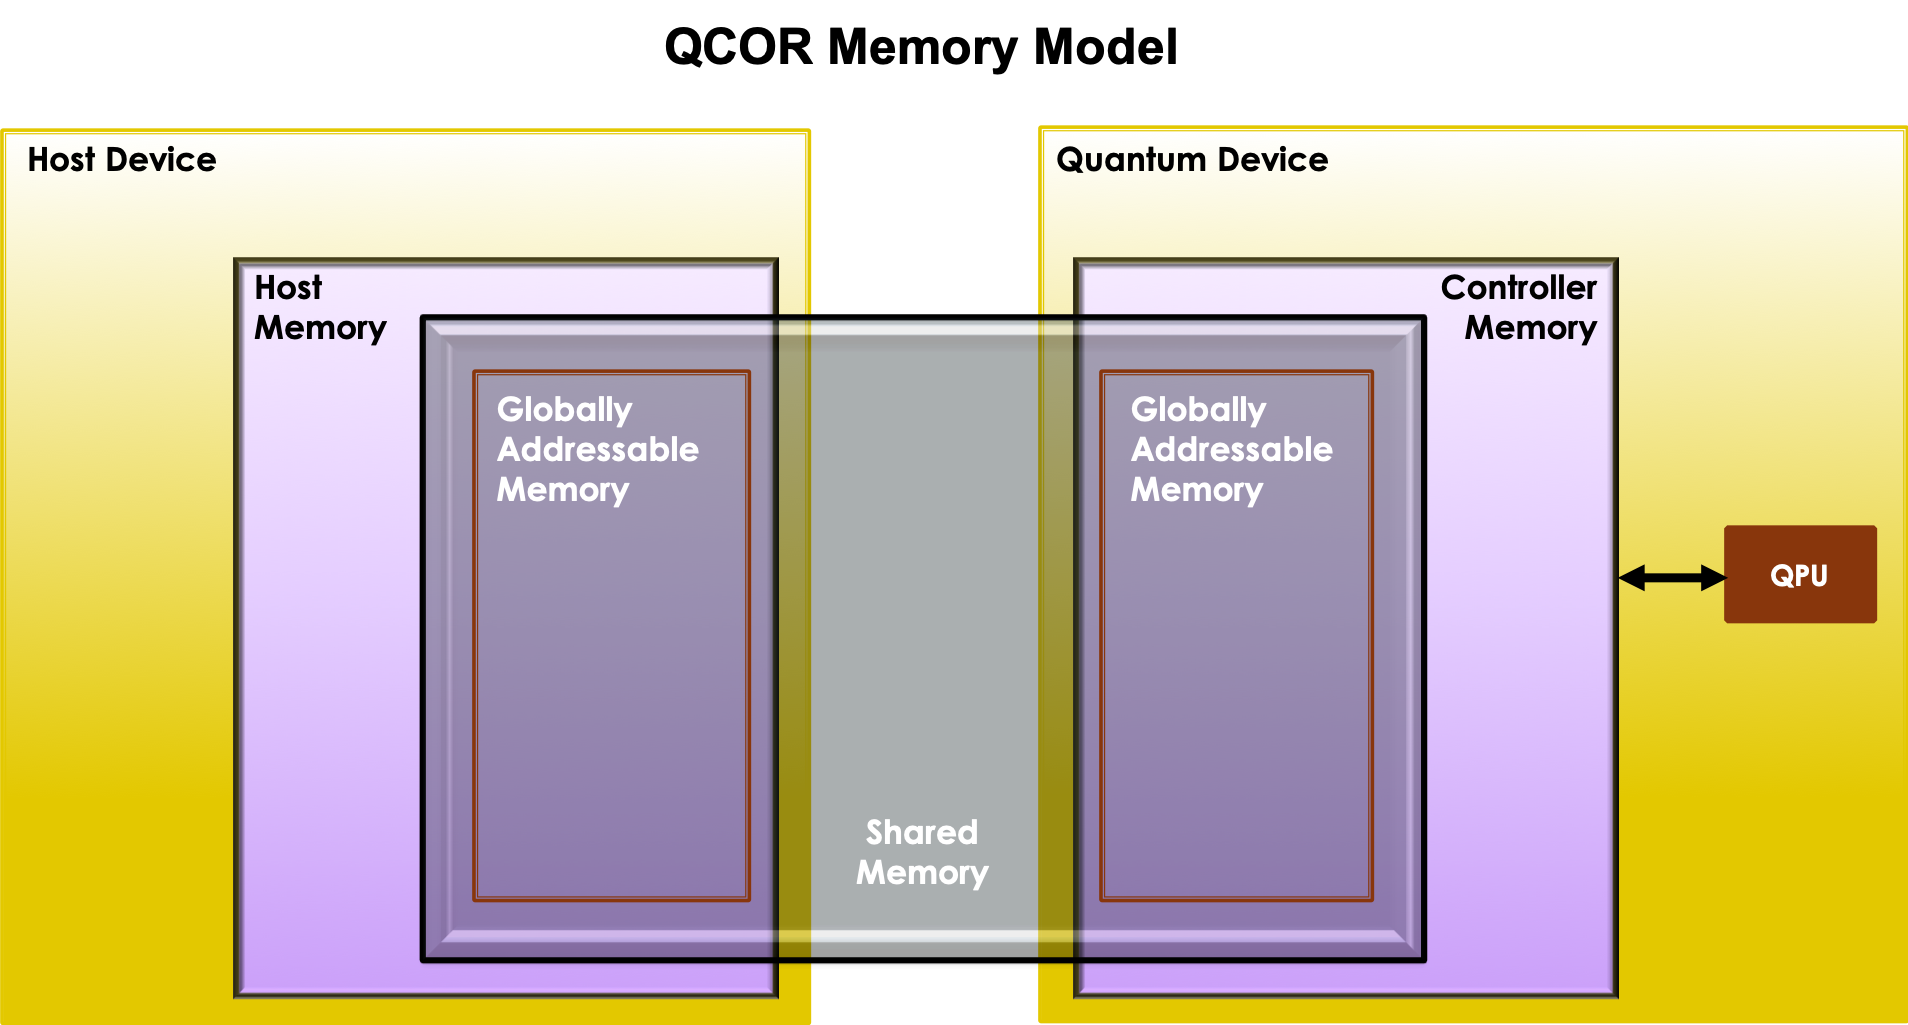
\includegraphics[height=3.5in,width=5.5in]{figures/Memory_Model_Illustration_v4.png}
  \caption{Diagram of the \qcor memory model}
  \label{fig:mem_model}
\end{figure*}


\section{Execution Model}\label{subsec:execution_model}
\qcor targets an execution model whereby application execution is directed by the host with access to an attached quantum device. Applications consist of purely classical and quantum-classical expressions and routines. Figure \ref{fig:exec_model} illustrates \qcor's execution model. Applications are compiled and execute both host and quantum device code. The host device executes \qcor library calls which may consist of both classical and quantum tasks. When the host encounters a quantum kernel within the quantum-classical task, the kernel is passed to the quantum device controller. \qcor quantum-classical tasks are executed asynchronously, meaning, the host initiates the task and continues to the next statement or expression in the application without waiting for the quantum-classical task to complete.
% Execution on the host is asynchronous to execution on the quantum device. 
\qcor exposes initialization, synchronization, execution, and memory management library application programming interfaces (api's) to the user that enable a wide variety of hybrid quantum-classical use cases.

\begin{figure*}
 \centering
 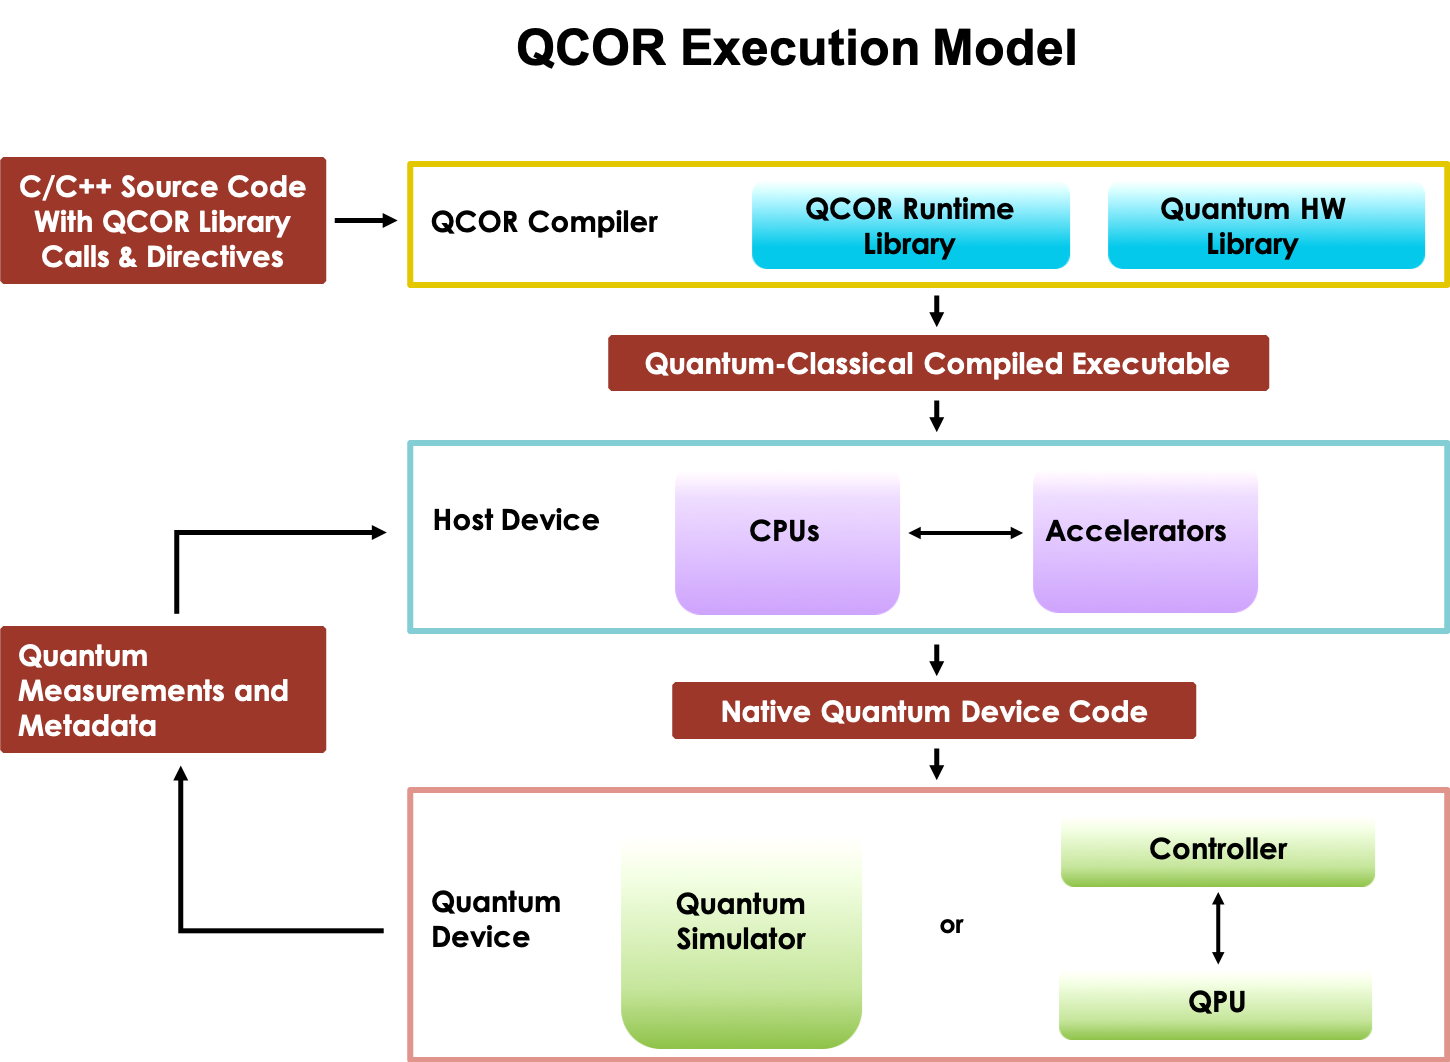
\includegraphics[width=5in,height=4in]{figures/Execution_Model_Illustration_v3.png}
  \caption{Diagram of \qcor Execution Model}
  \label{fig:exec_model}
\end{figure*}


\subsection{\textbf{Quantum Kernels}}\label{subsec:kernel}
\qcor extends \CorCpp by allowing the programmer to define functions, called \FUNC{kernels}, that, when called, are executed asynchronously on the quantum device. A \FUNC{kernel} is defined using the \_\_qpu\_\_ declaration specifier. A \FUNC{kernel} can optionally accept native or user defined \CorCpp datatypes as arguments, as well as datatypes within the \qcor language extension.

The \FUNC{kernel} function body should be a sequence of instructions on qbits and can also include control flow statements and predefined macros.  This circuit level expressiveness can be implemented using languages like \textit{QASM}, \textit{XASM}, and \textit{Quill}. 
%TODO: Insert footnotes or citations for qasm, xasm and quill

%The sample code below illustrates \FUNC{kernel} usage in a \CorCpp program.
%TODO: insert example


\section{Datatypes}\label{subsec:datatypes}
The \qcor specification has a set of datatypes that enable the expression of quantum concepts within the \qcor \ac{API}s.\\

\subsection{\textbf{ObjectiveFunction}}\label{subsec:ObjectiveFunction}
\DATATYPENAME{ObjectiveFunction} captures the behavior of a parameterizable function. The \DATATYPENAME{ObjectiveFunction} is initialized with the problem-specific observable and kernel. The \DATATYPENAME{ObjectiveFunction} also exposes a method to evaluate the kernel, given a set of parameters, and executes general pre- and post-processing of the kernel execution.\\
%SP 8/4/2020: Can we provide an example of an ObjectiveFunction?
%SP 8/4/2020: ''initialized with the problem-specific observable and kernel'' - this is confusing for someone new to the field, we just talked about it being a parameterizable function and then jump to an observable and kernel which are not yet defined.
%SP 8/4/2020: ''executes general pre- and post-processing of the kernel execution'' - executes [blah blah] of an execution - this doesn't really help understand the concept, perhaps could we reword?

\subsection{\textbf{Optimizer}}\label{subsec:Optimizer}
\DATATYPENAME{Optimizer} .\\


\subsection{\textbf{ResultsBuffer}}\label{subsec:ResultsBuffer}
\DATATYPENAME{ResultsBuffer} contains the measurement results from a single quantum execution.\\

\subsection{\textbf{Operator}}\label{subsec:Operator}
% description of how to build/initialize observable should be refined. 
\DATATYPENAME{Operator} is an operator built from Pauli Operators and Field Operators.
% does this refer to the underlying operator transformations?
It contains the data to algebraically relate basic and complex operations, 
% i.e. how we put together the observable from a set of non-commuting measurement bases
%SP 8/4/2020: agree with above comments, could we give an example as well?  Overall this explanation doesn't help me really understand what an observable is.
and the measurements from the observation of the kernel execution.\\
% is a pauli operator a subclass of a observable? consensus? should explicitely state if so. 

%\subsection{\textbf{PauliOperator}}\label{subsec:PauliOperator}
%\DATATYPENAME{PauliOperator} is a single operator type with three attributes: PauliX, PauliY or PauliZ, site/spatial index which is an %integer value, coefficient float value.\\

%\subsection{\textbf{FieldOperator}}\label{subsec:FieldOperator}
%\DATATYPENAME{FieldOperator} is a single operator type with four attributes: creator or anihilator, exchangeStatistics, site/spatial index %(which is an integer value), and a multiplicative complex scalar coefficient.\\

\subsection{\textbf{SiteMap}}\label{subsec:Sitemap}
% is this a mapping between a coodinate system (given a dimensionality) and indicies for the lattice sites? 
\DATATYPENAME{SiteMap} has an integer, \VAR{site_idx}, and string, \VAR{axis}, attribute. These attributes form a mapping of \VAR{site_idx} to \VAR{axis} for use in \Clang.

\subsection{\textbf{OperatorTransform}}\label{subsec:OperatorTransform}
\DATATYPENAME{OperatorTransform} A function mapping an (variatic number of) input Operator(s) to a transformed output (list of) Operator(s). 

\subsection{\textbf{HeterogeneousMap}}\label{subsec:HeterogeneousMap}
\DATATYPENAME{HeterogeneousMap} has two attributes a string \VAR{s} and void pointer \VAR{p} for use in \Clang.

\subsection{\textbf{qreg}}\label{subsec:qreg}
\DATATYPENAME{qreg} is the datatype representation for qubits.


%\section{Language Bindings and Conformance}\label{subsec:bindings}
%\input{content/language_bindings_and_conformance}

%\section{Library Constants}\label{subsec:library_constants}
%\input{content/library_constants}

%\section{Environment Variables }\label{subsec:environment_variables}
%\input{content/environment_variables}




\clearpage



\section{\qcor Library API}\label{sec:qcor_library_api}
\subsection{\textbf{taskInitiate}}\label{subsec:taskInitiate}
\apisummary{
 Invoked on the host to launch a quantum kernel on the quantum device.   
}

\begin{apidefinition}

\begin{Csynopsis}
Handle taskInitiate(ObjectiveFunction *objective, Optimizer *optimizer)
%SP 8/4/2020: fix text wrap so it doesn't cut at odd place
\end{Csynopsis}

\begin{Cppsynopsis}
Handle qcore::taskInitiate(ObjectiveFunction &objective, Optimizer &optimizer)
\end{Cppsynopsis}


\begin{apiarguments}
    \apiargument{IN}{objective}{A parameterized user defined function transforming input data into an output result}
    %SP 8/4/2020: how is this different from objectiveFunction?  the description is basically saying it is an objective function.  This has often confused me. EZJ ditto. 
    \apiargument{IN}{optimizer}{Takes an objective function as input and outputs the optimal function parameters and associated function value}
\end{apiarguments}

\apidescription{
The taskInitiate call is invoked on the host to launch a quantum kernel on the quantum device. The taskInitiate call references the objective function, and the classical optimizer. After a quantum kernel has been launched, host execution continues until the host reaches a sync call.  
}

\apireturnvalues{
    Handle for the quantum kernel launched by the taskInitiate call.
}      

\apinotes{
The taskInitiate call kicks off a hybrid quantum-classical task. For example, 
in variational quantum computing the kernel executes on the quantum 
device and the implementation may iterate         
execution between the quantum and classical
host devices, with the host performing classical optimization based on 
measurements from the quantum device.   
}

\end{apidefinition}


\subsection{\textbf{sync}}\label{subsec:sync}
\apisummary{
    
}

\begin{apidefinition}

\begin{Csynopsis}
    ResultsBuffer* sync(Handle qh)
\end{Csynopsis}

\begin{Cppsynopsis}
    ResultsBuffer* sync(Handle qh)
\end{Cppsynopsis}


\begin{apiarguments}
    \apiargument{IN}{qh}{Handle for the quantum kernel launched by the TaskInitiate call}
\end{apiarguments}

\apidescription{
    This a blocking execution call.  The sync call is initiated from the host device.  It blocks until the terminating condition of the objective function has been met.
}

\apireturnvalues{
    Returns an instance of \DATATYPENAME{ResultsBuffer} which contains output of the quantum kernel execution.
}      

\apinotes{
    
}

\end{apidefinition}


\subsection{\textbf{execute}}\label{subsec:execute}
\apisummary{
    
}

\begin{apidefinition}

\begin{Csynopsis}
    void execute (Handle *hdl)
\end{Csynopsis}

\begin{Cppsynopsis}
    void qcor::execute (Handle *hdl)
\end{Cppsynopsis}


\begin{apiarguments}
    \apiargument{IN}{hdl}{Handle created from the initial taskInitiate call.}
\end{apiarguments}

\apidescription{
    This re-executes the quantum kernel associated from a previous taskInitiate and sync which have already been called. Requires a subsequent sync call to retrieve results of re-execution.  
    %SP 8/4/2020: I'm confused by this descption.  
    % 'the quantum kernel associated' - with what?
    % why re-execute?
    % what does it return? nothing?
}

\apireturnvalues{
    
}      

\apinotes{
    
}

\end{apidefinition}


\subsection{\textbf{transform}}\label{subsec:transform}
\apisummary{
    Method transforming FieldOperators to a observable.
}

\begin{apidefinition}

\begin{Csynopsis}
Observable observableTransform(FieldOperator* fieldOp, void* modifier)
\end{Csynopsis}

\begin{Cppsynopsis}
Observable observableTransform(map<FieldOperator, FieldOperator> fieldOp, void* modifier)
%SP 8/4/2020: line wrap issue in pdf
\end{Cppsynopsis}


\begin{apiarguments}
    \apiargument{IN}{fieldOp}{list of variables of FieldOperator type}
    \apiargument{IN}{modifier}{a transformation mapping generalized operators to observables. This is a function pointer that implements transformations to observable produced by \FUNC{observableTransform}. The function header should accept the Observable type}
    %SP 8/4/2020: pauli or Pauli?
    %SP 8/4/2020: so the output of observableTransform can be modified by the modifier before being returned? Is this the right way to say/do this?
    %EZJ: also confused 
    \apiargument{OUT}{oberservable}{}
\end{apiarguments}

\apidescription{
    
}

\apireturnvalues{
    use shmem tex files as a guide
}      

\apinotes{
    
}

\begin{apiexamples}

\apicppexample
    { This is a simple program that calls \FUNC{observableTransform}: } 
    { example_code/transform_ex.cpp} 
    {}

\end{apiexamples}

\end{apidefinition}



\subsection{Memory Management Routines}
\subsubsection{\textbf{createResultsBuffer}}\label{subsec:createresbuf}
\apisummary{
    
}

\begin{apidefinition}

\begin{Csynopsis}

\end{Csynopsis}

\begin{Cppsynopsis}

\end{Cppsynopsis}


\begin{apiarguments}
    \apiargument{}{}{}
\end{apiarguments}

\apidescription{
    
}

\apireturnvalues{
    use shmem tex files as a guide
}      

\apinotes{
    
}

\begin{apiexamples}

\apicppexample
    { This is a simple program that calls \FUNC{createResultBuffer}: } 
    { example_code/createResultBuffer_ex.cpp} 
    {}

\end{apiexamples}

\end{apidefinition}


\subsubsection{\textbf{createObservable}}\label{subsec:createobserv}
\apisummary{
    Creates an observable
}

\begin{apidefinition}

\begin{Csynopsis}
    Observable* createObservable (SiteMap *sitemap, double complex coef)
\end{Csynopsis}

\begin{Cppsynopsis}
    Observable* qcor::createObservable (std::map<int,string> sitemap, std::complex coef)
\end{Cppsynopsis}


\begin{apiarguments}
    \apiargument{IN}{sitemap}{mapping of an integer to a string of value``x'', ``y'' or ``z''}
    \apiargument{IN}{coef}{coefficient for sitemap terms}
\end{apiarguments}

\apidescription{
        \FUNC{createObservable} accepts an integer:string mapping, \VAR{sitemap}, of an integer site number to a string ``x'', ``y'', or ``z''. \VAR{sitemap} may contain one or more integer:string mappings. The complex coefficient \VAR{coef} argument can optionally be included to multiply each term in the site map. If \VAR{coef} is not included, the default value is 1.
}

\apireturnvalues{
    Returns a pointer to a new \DATATYPENAME{Observable}. 
}      

\apinotes{
    The interger:string mapping has a seperate datatype representation for \Clang and \Cpp. The \Clang representation is a \qcor library type, \DATATYPENAME{SiteMap}.  The \Cpp representation is the \Cpp standard library type \DATATYPENAME{map}. 
 %SP 8/4/2020: space after \Clang ? 
    %EZJ: Does one need to createobserve(fieldOp) and then use observableTransform(fieldOp) to populate the observable with data?
    %i.e. we need to specify and deliniate the relationship between createobserve and observableTransform. 
}

\begin{apiexamples}

\apicppexample
    { This is a simple program that calls \FUNC{createObservable}: } 
    { example_code/createObservable_ex.cpp} 
    {}

\end{apiexamples}

\end{apidefinition}


\subsubsection{\textbf{createPauli}}\label{subsec:createpauli}
\apisummary{
    
}

\begin{apidefinition}

\begin{Csynopsis}
    
\end{Csynopsis}

\begin{Cppsynopsis}
    
\end{Cppsynopsis}


\begin{apiarguments}
    \apiargument{IN}{sitemap}{mapping of integer 'key' to a string of value "x", "y" or "z"}
    \apiargument{IN}{paulistr}{string}
    \apiargument{IN}{coef}{coefficient}
\end{apiarguments}

\apidescription{
        \FUNC{createPauli} accepts a string representation of a complex Pauli operator, \VAR{paulistr}, or an integer:string mapping, \VAR{sitemap}, of an integer site number to a string "x", "y", or "z". The integer \VAR{coef} argument can optionally be included with \VAR{sitemap} to multiply each term in the site map. If \VAR{coef} is not included, the default value is 1.
        - if empty map, is an identity
        - map is any integer index to string x, y or z
        - coefficient optional, defaults to 1
        - string composition/concatenation of the form "<coefficient> <pauli string> <integer> ... <optional operation>"
}

\apireturnvalues{
    
}      

\apinotes{
 The interger:string mapping has a seperate datatype representation for \Clang and \Cpp. The \Clang representation is a \qcor library type, \DATATYPENAME{SiteMap}.  The \Cpp representation is the \Cpp standard library type \DATATYPENAME{map}.  
}

\begin{apiexamples}

\apicppexample
    { This is a simple program that calls \FUNC{createPauli}: } 
    { example_code/createPauli_ex.cpp} 
    {}

\end{apiexamples}

\end{apidefinition}


\subsubsection{\textbf{pauliX}}\label{subsec:paulix}
\apisummary{
    Creates a Pauli X operator at site n.   
}

\begin{apidefinition}

\begin{Csynopsis}
    PauliOperator pauliX(int n)
\end{Csynopsis}

\begin{Cppsynopsis}
    PauliOperator qcor::pauliX(int n)
\end{Cppsynopsis}


\begin{apiarguments}
    \apiargument{IN}{n}{integer value}
\end{apiarguments}

\apidescription{
       \FUNC{pauliX} accepts an integer input that creates a Pauli X operator at site n.  The Pauli X operator is returned as a \DATATYPENAME{PauliOperator}.
}

\apireturnvalues{
    returns PauliOperator for pauliX
}      

\apinotes{
    
}

\begin{apiexamples}

\apicppexample
    { This is a simple program that calls \FUNC{pauliX}: } 
    { example_code/pauliX_ex.cpp} 
    {}

\end{apiexamples}

\end{apidefinition}


\subsubsection{\textbf{pauliY}}\label{subsec:pauliy}
\apisummary{
    
}

\begin{apidefinition}

\begin{Csynopsis}
    
\end{Csynopsis}

\begin{Cppsynopsis}
    
\end{Cppsynopsis}


\begin{apiarguments}
    \apiargument{}{}{}
\end{apiarguments}

\apidescription{
        
}

\apireturnvalues{
    
}      

\apinotes{
    
}

\begin{apiexamples}

\apicppexample
    { This is a simple program that calls \FUNC{pauliY}: } 
    { example_code/pauliY_ex.cpp} 
    {}

\end{apiexamples}

\end{apidefinition}


\subsubsection{\textbf{pauliZ}}\label{subsec:pauliz}
\apisummary{
     Creates Pauli Z operator at site n.
}

\begin{apidefinition}

\begin{Csynopsis}
    Operator pauliZ(int n)
\end{Csynopsis}

\begin{Cppsynopsis}
    Operator qcor::pauliZ(int n)
\end{Cppsynopsis}


\begin{apiarguments}
    \apiargument{IN}{n}{integer value}
\end{apiarguments}

\apidescription{
        \FUNC{pauliZ} accepts an integer input that creates a Pauli Z operator at site \VAR{n}.
}

\apireturnvalues{
    Returns a single instance of \DATATYPENAME{Operator}.
}      

\apinotes{
    
}

\end{apidefinition}


\subsubsection{\textbf{createFieldOp}}\label{subsec:createfieldop}
\apisummary{
    creates a Bosonic or Fermionic field operator
}

\begin{apidefinition}

\begin{Csynopsis}
    Operator* createFieldOp(char* opType, char* relType, int siteIdx, double complex coef)
\end{Csynopsis}

\begin{Cppsynopsis}
    Operator* qcor::createFieldOp(string opType, string relType, int siteIdx, std::complex coef)
\end{Cppsynopsis}


\begin{apiarguments}
    \apiargument{IN}{opType}{a string that designates if the field operator is a creation or annihilation operator}
    \apiargument{IN}{relType}{a string that designates if the commutation relations are either Fermionic or Bosonic}
    \apiargument{IN}{siteIdx}{integer site index}
    \apiargument{IN}{coef}{complex coefficient value}
\end{apiarguments}

\apidescription{
        \FUNC{createFieldOp} creates a creation or annihilation field operator representation that is either Fermionic or Bosonic. The creation or annihilation atrribute is set by assigning the string value ``create'' or ``annihilate'', respectively, to \VAR{opType}.  The Fermionic or Bosonic attribute is set by assigning the string value ``Fermion'' or ``Boson'', respectively, to \VAR{relType}. \FUNC{createFieldOp} must also assign an integer site index via \VAR{sizeIdx}. The complex coefficient \VAR{coef} is optional, and is 1 by default. 
}

\apireturnvalues{
    Returns a pointer to a single instance of \DATATYPENAME{Operator}.
}      

\apinotes{
    
}

\end{apidefinition}



\subsection{Algebraic Routines}
\subsubsection{\textbf{addOperation}}\label{subsec:addop}
\apisummary{
   Takes Observables and returns their sum. 
}

\begin{apidefinition}

\begin{Csynopsis}
    Obervable* addOperation(Observable* op1, Observable* op2, ...)
\end{Csynopsis}

\begin{Cppsynopsis}
    Obervable* qcor::addOperation(Observable &op1, Observable &op2, ...)
\end{Cppsynopsis}


\begin{apiarguments}
    \apiargument{IN}{op1}{first Observable operand}
    \apiargument{IN}{op2}{second Observable operand}
    \apiargument{IN}{...}{additional Observable operand}
\end{apiarguments}

\apidescription{
        The \FUNC{addOperation} routine adds two or more \DATATYPENAME{Observables}.
}

\apireturnvalues{
    Returns a new instance of \DATATYPENAME{Observable}.
}      

\apinotes{
    
}

\begin{apiexamples}

\apicppexample
    { This is a simple program that calls \FUNC{addOperation}: } 
    { example_code/addOperation_ex.cpp} 
    {}

\end{apiexamples}

\end{apidefinition}


\subsubsection{\textbf{multiplyOperation}}\label{subsec:mulop}
\apisummary{
    
}

\begin{apidefinition}

\begin{Csynopsis}
    
\end{Csynopsis}

\begin{Cppsynopsis}
    
\end{Cppsynopsis}


\begin{apiarguments}
    \apiargument{}{}{}
\end{apiarguments}

\apidescription{
        
}

\apireturnvalues{
    
}      

\apinotes{
    
}

\begin{apiexamples}

\apicppexample
    { This is a simple program that calls \FUNC{multiplyOperation}: } 
    { example_code/multiplyOperation_ex.cpp} 
    {}

\end{apiexamples}

\end{apidefinition}


\subsubsection{\textbf{mergeOperation}}\label{subsec:mergeop}
\apisummary{
    
}

\begin{apidefinition}

\begin{Csynopsis}
    
\end{Csynopsis}

\begin{Cppsynopsis}
    
\end{Cppsynopsis}


\begin{apiarguments}
    \apiargument{}{}{}
\end{apiarguments}

\apidescription{
        
}

\apireturnvalues{
    
}      

\apinotes{
    
}

\begin{apiexamples}

\apicppexample
    { This is a simple program that calls \FUNC{mergeOperation}: } 
    { example_code/mergeOperation_ex.cpp} 
    {}

\end{apiexamples}

\end{apidefinition}



\clearpage



\clearpage

\appendix

%defining pagestyle for annex
%\pagestyle{plain} \withlinenumbers
\pagestyle{fancy} \withlinenumbers
\fancyhf{}
\fancyhead[RE, LO]{\leftmark}
\fancyhead[RO, LE]{\thepage}
\fancyfoot[CE,CO]{\thepage}
\renewcommand{\headrulewidth}{0pt}




\chapter{Writing \qcor Programs}
\section*{Incorporating \qcor{} into Programs}\label{sec:writing_programs}



\chapter{Compiling and Running Programs}\label{sec:compiling}

\section{Compilation}
\subsection*{Programs written in \Clang}


\subsection*{Programs written in \Cpp}

%\subsection*{Programs written in \Python}


\section{Running Programs}





\chapter{Undefined Behavior in \qcor}\label{sec:undefined}





\chapter{Interoperability with other Programming Models}\label{sec:interop}



\clearpage












%\chapter{Changes to this Document}\label{sec:changelog}


%\section{Version x.x}

%The following list describes the specific changes in x.x:

%\begin{itemize}
%\end{itemize}







} %end of setlength command that was started in frontmatter.tex



\end{document}

